\documentclass[aspectratio=169,10pt]{beamer}

\usetheme{Madrid}
\setbeamertemplate{navigation symbols}{}
\setbeamertemplate{footline}[frame number]

\usepackage{booktabs}
\usepackage{tabularx}
\usepackage{array}
\usepackage{ragged2e}
\usepackage{xcolor}
\usepackage{tikz}
\usepackage{pgfplots}
\usepgfplotslibrary{groupplots}
\usetikzlibrary{arrows.meta,positioning,shapes.geometric,fit}

\pgfplotsset{compat=1.18}

\definecolor{cfblue}{HTML}{1F4E79}
\definecolor{cflight}{HTML}{EAF2F8}
\definecolor{cfaccent}{HTML}{B54A3A}
\definecolor{cfgreen}{HTML}{2F6B3C}
\definecolor{cfgray}{HTML}{5B6570}
\definecolor{cforange}{HTML}{D78B28}
\definecolor{cfpurple}{HTML}{6D5BA6}

\setbeamercolor{structure}{fg=cfblue}
\setbeamercolor{title}{fg=cfblue}
\setbeamercolor{frametitle}{fg=cfblue,bg=cflight}
\setbeamercolor{block title}{fg=white,bg=cfblue}
\setbeamercolor{block body}{bg=black!3}
\setbeamercolor{alerted text}{fg=cfaccent}

\newcolumntype{Y}{>{\RaggedRight\arraybackslash}X}
\newcommand{\sources}[1]{\vfill{\tiny\color{cfgray}Source(s): #1}}

\title{CARD Progress Report}
\subtitle{Research-focused window: 24 Mar 2026 -- 06 Apr 2026}
\author{Repository progress summary}
\institute{Built from git history, repo benchmark notes, and funded benchmark records through 03 Apr 2026}
\date{06 Apr 2026}

\begin{document}

\begin{frame}
  \titlepage
\end{frame}

\begin{frame}{Reporting scope: research-valid progress after 24 Mar 2026}
\small
\begin{itemize}
  \item This report excludes earlier March tuning work and focuses on results that strengthened the \textbf{research case}, not only the codebase.
  \item Three themes dominate this window: \textbf{measurement validity}, \textbf{before/after evidence}, and a \textbf{more robust funded benchmark design}.
\end{itemize}

\vspace{0.4em}
\centering
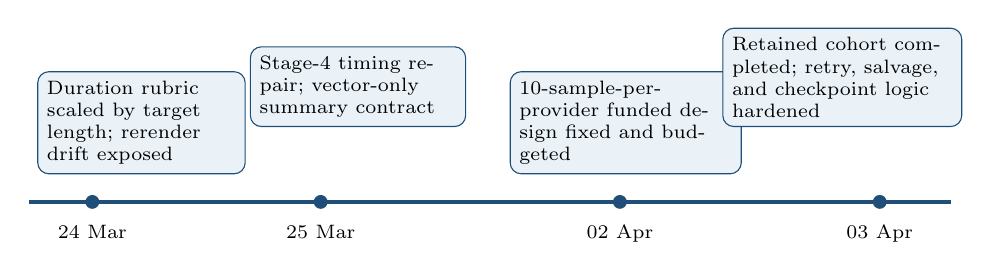
\begin{tikzpicture}[x=1cm,y=1cm,>=Latex]
  \draw[cfblue,very thick] (0,0) -- (11.7,0);
  \foreach \x/\label in {
    0.8/{24 Mar},
    3.7/{25 Mar},
    7.5/{02 Apr},
    10.8/{03 Apr}
  } {
    \fill[cfblue] (\x,0) circle (2.5pt);
    \node[font=\scriptsize,below=5pt] at (\x,0) {\label};
  }
  \node[draw=cfblue,rounded corners,fill=cflight,align=left,font=\scriptsize,anchor=south west,text width=2.4cm] at (0.1,0.35)
    {Duration rubric scaled by target length; rerender drift exposed};
  \node[draw=cfblue,rounded corners,fill=cflight,align=left,font=\scriptsize,anchor=south west,text width=2.5cm] at (2.8,0.95)
    {Stage-4 timing repair; vector-only summary contract};
  \node[draw=cfblue,rounded corners,fill=cflight,align=left,font=\scriptsize,anchor=south west,text width=2.7cm] at (6.1,0.35)
    {10-sample-per-provider funded design fixed and budgeted};
  \node[draw=cfblue,rounded corners,fill=cflight,align=left,font=\scriptsize,anchor=south west,text width=2.8cm] at (8.8,0.95)
    {Retained cohort completed; retry, salvage, and checkpoint logic hardened};
\end{tikzpicture}

\sources{coder\_docs/memory/errors\_and\_notes.md; coder\_docs/sporc\_budget\_reference\_20260402.md; git log since 2026-03-24}
\end{frame}

\begin{frame}{Why the new benchmark is more research-worthy}
\small
\begin{columns}[T,totalwidth=\textwidth]
\column{0.56\textwidth}
\begin{block}{24 Mar evidence base vs 02--03 Apr evidence base}
{\scriptsize
\begin{tabularx}{\linewidth}{p{1.9cm}YY}
\toprule
 & 24 Mar DeepSeek bundle & 02--03 Apr retained cohort \\
\midrule
Design & 5 episodes \(\times\) 3 presets = 15 outputs & 10 retained samples \emph{per provider} \\
Provider scope & DeepSeek only & Anthropic, DeepSeek, vLLM, OpenAI \\
What it proved & End-to-end feasibility and duration range & Matched cross-provider benchmark evidence \\
Completion & 15/15 outputs completed & 40/40 retained samples completed \\
\bottomrule
\end{tabularx}
}
\end{block}

\column{0.44\textwidth}
\centering
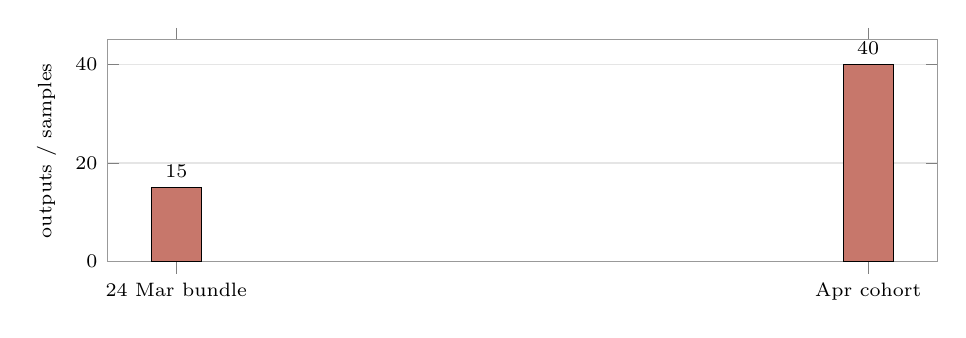
\begin{tikzpicture}
\begin{axis}[
  width=\linewidth,
  height=4.4cm,
  ybar,
  bar width=18pt,
  ymin=0,ymax=45,
  symbolic x coords={24 Mar bundle,Apr cohort},
  xtick=data,
  xticklabel style={font=\scriptsize,align=center},
  nodes near coords,
  nodes near coords style={font=\scriptsize},
  ylabel={outputs / samples},
  tick label style={font=\scriptsize},
  label style={font=\scriptsize},
  axis line style={draw=black!40},
  ymajorgrids,
  grid style={black!10}
]
\addplot[fill=cfaccent!75] coordinates {(24 Mar bundle,15) (Apr cohort,40)};
\end{axis}
\end{tikzpicture}

\vspace{-0.5em}
{\scriptsize April cohort transcripts: 17.2k--31.8k words, mean 20.7k.}
\end{columns}

\sources{research/paper/sections/05\_stage3.tex:49--67; coder\_docs/sporc\_budget\_reference\_20260402.md:7--16, 210--219, 304--324}
\end{frame}

\begin{frame}{Proof 1: duration validity improved after the rerender-drift bug}
\small
\begin{columns}[T,totalwidth=\textwidth]
\column{0.54\textwidth}
\begin{block}{Bad behavior observed on 24 Mar}
\begin{itemize}
  \item A critic-approved live draft measured \textbf{30.77 s}.
  \item Forced stage-3 rerender turned the merged export into \textbf{33.01 s}.
  \item That is \textbf{+2.24 s drift} or about \textbf{+7.3\%} relative to the approved draft.
\end{itemize}
\end{block}

\begin{alertblock}{Why this matters for research}
If the exported audio no longer matches the draft that the critic approved, then reported duration adherence becomes methodologically weak.
\end{alertblock}

\column{0.46\textwidth}
\centering
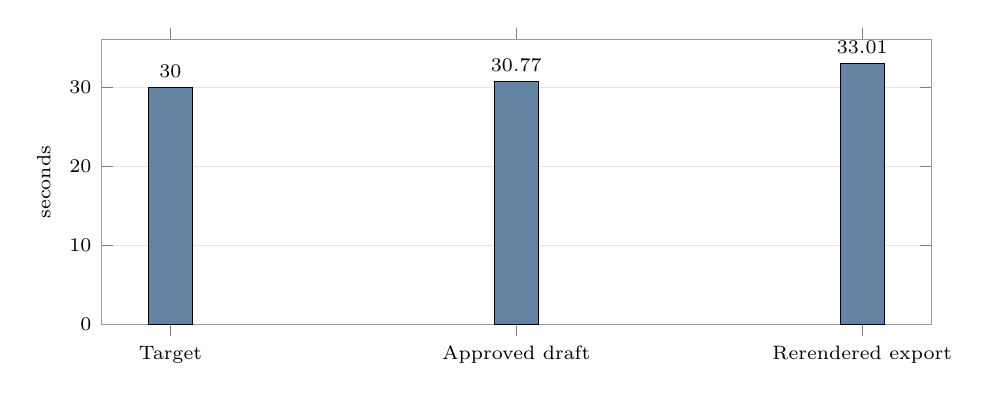
\begin{tikzpicture}
\begin{axis}[
  width=\linewidth,
  height=5.2cm,
  ybar,
  bar width=16pt,
  ymin=0,ymax=36,
  symbolic x coords={Target,Approved draft,Rerendered export},
  xtick=data,
  xticklabel style={font=\scriptsize,align=center},
  ylabel={seconds},
  label style={font=\scriptsize},
  tick label style={font=\scriptsize},
  nodes near coords,
  nodes near coords style={font=\scriptsize},
  ymajorgrids,
  grid style={black!10},
  axis line style={draw=black!40}
]
\addplot[fill=cfblue!70] coordinates {(Target,30) (Approved draft,30.77) (Rerendered export,33.01)};
\end{axis}
\end{tikzpicture}

{\scriptsize Fixed path: reuse the already measured live draft instead of rerendering it by default.}
\end{columns}

\sources{coder\_docs/memory/errors\_and\_notes.md:185--187}
\end{frame}

\begin{frame}{Proof 2: stage-4 overlap timing moved from audible lag to 0 ms residual onset}
\small
\begin{columns}[T,totalwidth=\textwidth]
\column{0.58\textwidth}
\centering
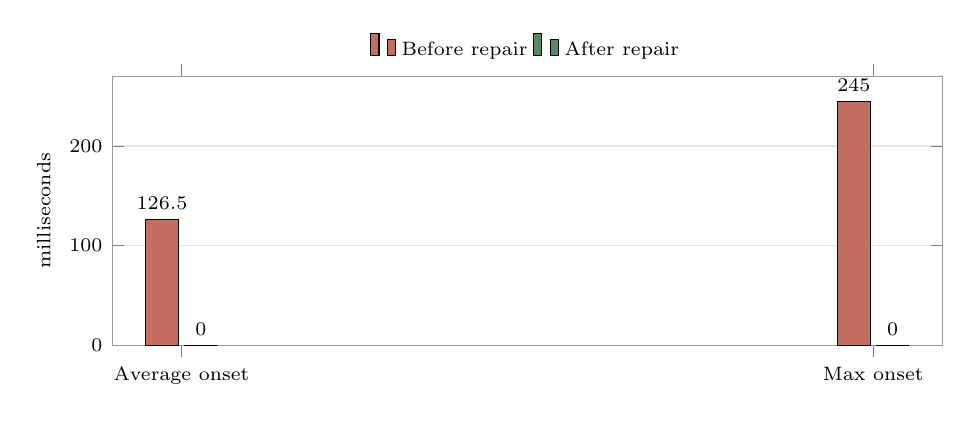
\begin{tikzpicture}
\begin{axis}[
  width=\linewidth,
  height=5cm,
  ybar,
  bar width=12pt,
  ymin=0,ymax=270,
  symbolic x coords={Average onset,Max onset},
  xtick=data,
  xticklabel style={font=\scriptsize,align=center},
  ylabel={milliseconds},
  label style={font=\scriptsize},
  tick label style={font=\scriptsize},
  legend style={font=\scriptsize,at={(0.5,1.02)},anchor=south,legend columns=2,draw=none},
  nodes near coords,
  nodes near coords style={font=\scriptsize},
  ymajorgrids,
  grid style={black!10},
  axis line style={draw=black!40}
]
\addplot[fill=cfaccent!80] coordinates {(Average onset,126.5) (Max onset,245)};
\addplot[fill=cfgreen!80] coordinates {(Average onset,0) (Max onset,0)};
\legend{Before repair,After repair}
\end{axis}
\end{tikzpicture}

\column{0.42\textwidth}
\begin{block}{Measured evidence}
\begin{itemize}
  \item Hidden leading silence was explicitly logged and trimmed.
  \item Example accepted trims: \textbf{190 ms}, \textbf{220 ms}, and \textbf{210 ms}.
  \item After repair, the remaining problems were semantic, not onset-related.
\end{itemize}
\end{block}

\begin{block}{Research takeaway}
This turned a subjective “the overlap sounds late” complaint into a measurable before/after result.
\end{block}
\end{columns}

\sources{coder\_docs/interjector\_timing\_refinement\_experiments\_20260325.md:310--327; coder\_docs/memory/errors\_and\_notes.md:121--123, 157--159}
\end{frame}

\begin{frame}{Retained 10-sample cohort: what the benchmark now shows}
\scriptsize
\begin{columns}[T,totalwidth=\textwidth]
\column{0.62\textwidth}
\centering
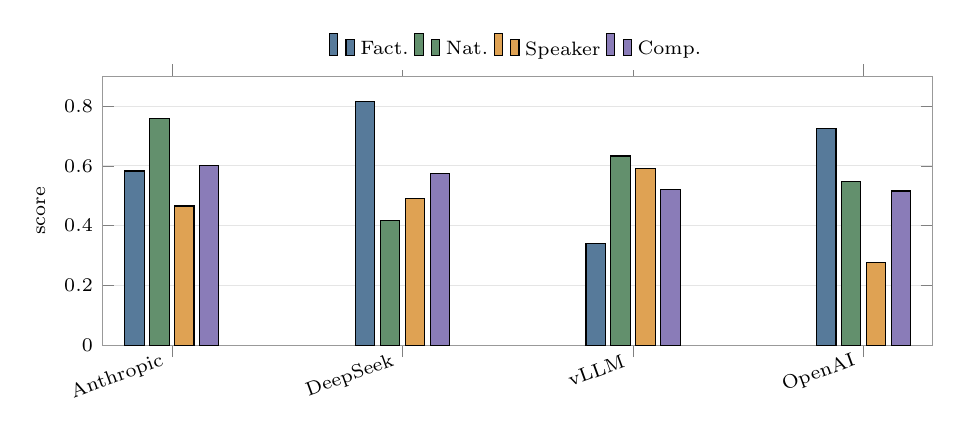
\begin{tikzpicture}
\begin{axis}[
  width=\linewidth,
  height=5cm,
  ybar,
  bar width=7pt,
  ymin=0,ymax=0.9,
  symbolic x coords={Anthropic,DeepSeek,vLLM,OpenAI},
  xtick=data,
  xticklabel style={font=\scriptsize,rotate=20,anchor=east},
  ylabel={score},
  label style={font=\scriptsize},
  tick label style={font=\scriptsize},
  legend style={font=\scriptsize,at={(0.5,1.02)},anchor=south,legend columns=4,draw=none},
  ymajorgrids,
  grid style={black!10},
  axis line style={draw=black!40}
]
\addplot[fill=cfblue!75] coordinates {(Anthropic,0.5830) (DeepSeek,0.8160) (vLLM,0.3406) (OpenAI,0.7240)};
\addplot[fill=cfgreen!75] coordinates {(Anthropic,0.7580) (DeepSeek,0.4160) (vLLM,0.6330) (OpenAI,0.5483)};
\addplot[fill=cforange!80] coordinates {(Anthropic,0.4660) (DeepSeek,0.4920) (vLLM,0.5920) (OpenAI,0.2763)};
\addplot[fill=cfpurple!80] coordinates {(Anthropic,0.6023) (DeepSeek,0.5746) (vLLM,0.5219) (OpenAI,0.5162)};
\legend{Fact., Nat., Speaker, Comp.}
\end{axis}
\end{tikzpicture}

\column{0.38\textwidth}
\centering
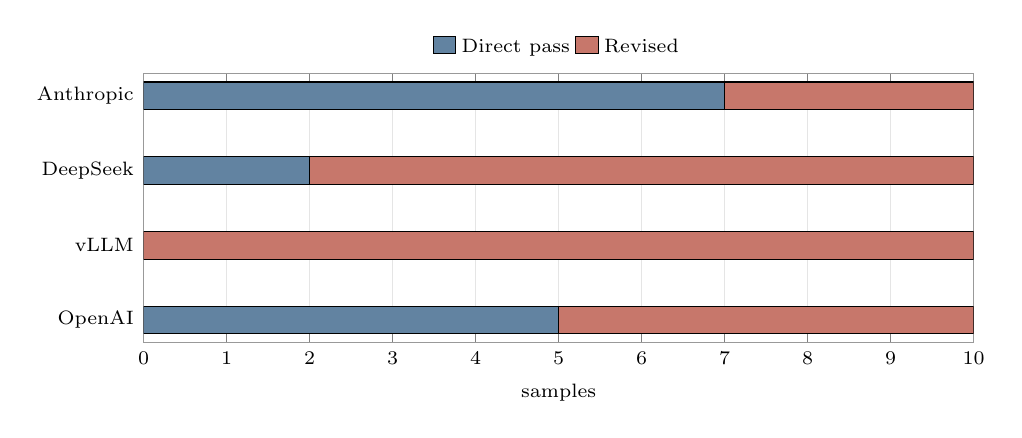
\begin{tikzpicture}
\begin{axis}[
  width=\linewidth,
  height=5cm,
  xbar stacked,
  xmin=0,xmax=10,
  symbolic y coords={Anthropic,DeepSeek,vLLM,OpenAI},
  ytick=data,
  y dir=reverse,
  tick label style={font=\scriptsize},
  label style={font=\scriptsize},
  xlabel={samples},
  legend style={font=\scriptsize,at={(0.5,1.02)},anchor=south,legend columns=2,draw=none},
  xmajorgrids,
  grid style={black!10},
  axis line style={draw=black!40}
]
\addplot[fill=cfblue!70] coordinates {(7,Anthropic) (2,DeepSeek) (0,vLLM) (5,OpenAI)};
\addplot[fill=cfaccent!75] coordinates {(3,Anthropic) (8,DeepSeek) (10,vLLM) (5,OpenAI)};
\legend{Direct pass,Revised}
\end{axis}
\end{tikzpicture}

\vspace{-0.3em}
\begin{block}{Reading the result}
\tiny Anthropic led overall; DeepSeek led factualness; vLLM led speaker-style fidelity; OpenAI stayed competitive on grounding but weak on speaker grammar.
\end{block}
\end{columns}

\sources{coder\_docs/sporc\_budget\_reference\_20260402.md:311--380}
\end{frame}

\begin{frame}{Threats to validity and how this window addressed them}
\small
\begin{columns}[T,totalwidth=\textwidth]
\column{0.58\textwidth}
\begin{block}{Observed threats during the funded run}
\begin{itemize}
  \item Provider rate limiting and hidden race conditions increased cost and endangered sample retention.
  \item Without checkpointed retries, the run could have finished with an uneven or biased cohort.
\end{itemize}
\end{block}

\begin{block}{Controls added in response}
\begin{itemize}
  \item Exact retained-sample targets instead of raw prefix counts.
  \item Resume-in-place after rate limits.
  \item Partial-draft checkpoints for interrupted samples.
  \item Cheap postprocess revision for capped runs that already had usable drafts.
\end{itemize}
\end{block}

\column{0.42\textwidth}
\centering
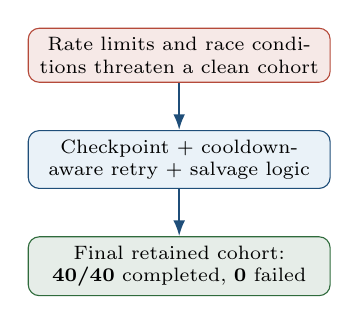
\begin{tikzpicture}[node distance=0.6cm]
  \node[draw=cfaccent,rounded corners,fill=cfaccent!12,align=center,text width=3.6cm,font=\scriptsize] (risk) {Rate limits and race conditions threaten a clean cohort};
  \node[draw=cfblue,rounded corners,fill=cflight,below=of risk,align=center,text width=3.6cm,font=\scriptsize] (control) {Checkpoint + cooldown-aware retry + salvage logic};
  \node[draw=cfgreen,rounded corners,fill=cfgreen!12,below=of control,align=center,text width=3.6cm,font=\scriptsize] (result) {Final retained cohort: \textbf{40/40} completed, \textbf{0} failed};
  \draw[-{Latex[length=2mm]},thick,cfblue] (risk) -- (control);
  \draw[-{Latex[length=2mm]},thick,cfblue] (control) -- (result);
\end{tikzpicture}

\vspace{0.5em}
\begin{block}{Budget note}
\scriptsize Estimated API spend for the funded design was about \$37.62, with a suggested \$48 buffer.
\end{block}
\end{columns}

\sources{coder\_docs/sporc\_budget\_reference\_20260402.md:35--48, 95--129, 180--204, 264--324}
\end{frame}

\begin{frame}{Conclusion and next research steps}
\small
\begin{block}{What this report can now claim}
\begin{itemize}
  \item Since 24 Mar, the project improved not only functionality but also \textbf{research defensibility}.
  \item Two concrete measurement bugs were turned into before/after evidence: duration drift and stage-4 onset lag.
  \item The strongest new result is the \textbf{retained 10-sample-per-provider benchmark}, which is a better basis for comparison than the earlier exploratory trials.
\end{itemize}
\end{block}

\begin{block}{Next steps}
\begin{itemize}
  \item Freeze the retained cohort and archive the exact benchmark configuration.
  \item Convert the 10-sample findings into participant-facing listening-study materials.
  \item Use the same retained-cohort discipline for future model comparisons instead of reverting to smaller ad hoc trials.
\end{itemize}
\end{block}

\sources{coder\_docs/sporc\_budget\_reference\_20260402.md; coder\_docs/memory/errors\_and\_notes.md; research/paper/sections/05\_stage3.tex}
\end{frame}

\end{document}
